\chapter{Theory}
\label{chp:theory}

\begin{center}
    \textit{This chapter delves into the theoretical foundations of the technologies and methodologies employed in the project. It covers key concepts such as computer vision, image recognition, and software engineering principles}    
\end{center}

\section{Literature Review}
\label{sec:literature-review}

As technology continues to evolve, a variety of digital tools and platforms have emerged to enhance the experience of playing and analyzing chess. Leading online platforms such as \textit{chess.com} and \textit{lichess.org} provide global matchmaking, tutorials, and advanced game analysis features. These innovations have transformed how chess is played and studied. \\

In parallel with these software-based innovations, physical chessboards and tournament practices have also been modernized through the integration of digital technologies. For instance, the use of \gls{rfid} enables the digitization of \gls{otb} games. \gls{rfid} works by embedding small tags in the chess pieces, which are detected by sensors in the board to identify each move \cite{quora:shah}. This approach bridges the gap between physical gameplay and digital analysis. \\

As an alternative to \gls{rfid}-based systems, electronic scoresheet solutions have been introduced to enable digital recording of chess games. One notable example is Clono, a tablet-based platform that transmits move data directly to a central server. The system supports live broadcasting of tournaments and offers a secure, low-cost, and user-friendly interface. By removing the need for electronic chessboards, physical cables, or on-site technical staff, Clono presents a practical and accessible solution for modern tournament management \cite{clono}. \\

Advancements in \gls{ai} have also enabled the development of tools that automate the digitization of chess games through visual recognition. A prominent example is \textit{ChessCam}, a web- and mobile-based application that processes video footage to detect moves and generate \gls{pgn} files \cite{github:chesscam, lichess:chesscam}. This approach makes it possible to digitize games with minimal hardware and manual work.

\section{Artificial Intelligence} 
\label{sec:artificial-intelligence}

\gls{ai} refers to the development of computer systems capable of performing tasks that typically require human intelligence, such as reasoning, problem-solving, perception, and language understanding. It encompasses a wide range of techniques and approaches aimed at replicating or augmenting human cognitive functions \cite{ibm:ai}. \\

A subfield of \gls{ai} is \gls{ml}, which focuses on enabling computers to learn from data and improve their performance on various tasks without being explicitly programmed. ML techniques are widely used in many AI applications due to their ability to generalize from examples. \\

One area where \gls{ai} and \gls{ml} are commonly applied is \textbf{computer vision}. This field enables machines to interpret, analyze, and extract meaningful information from visual data, such as digital images and videos. The primary goal of computer vision is to replicate the human ability to perceive and understand visual information, as illustrated in Figure~\ref{fig:computer-vision}.

\begin{figure}[h!] \centering 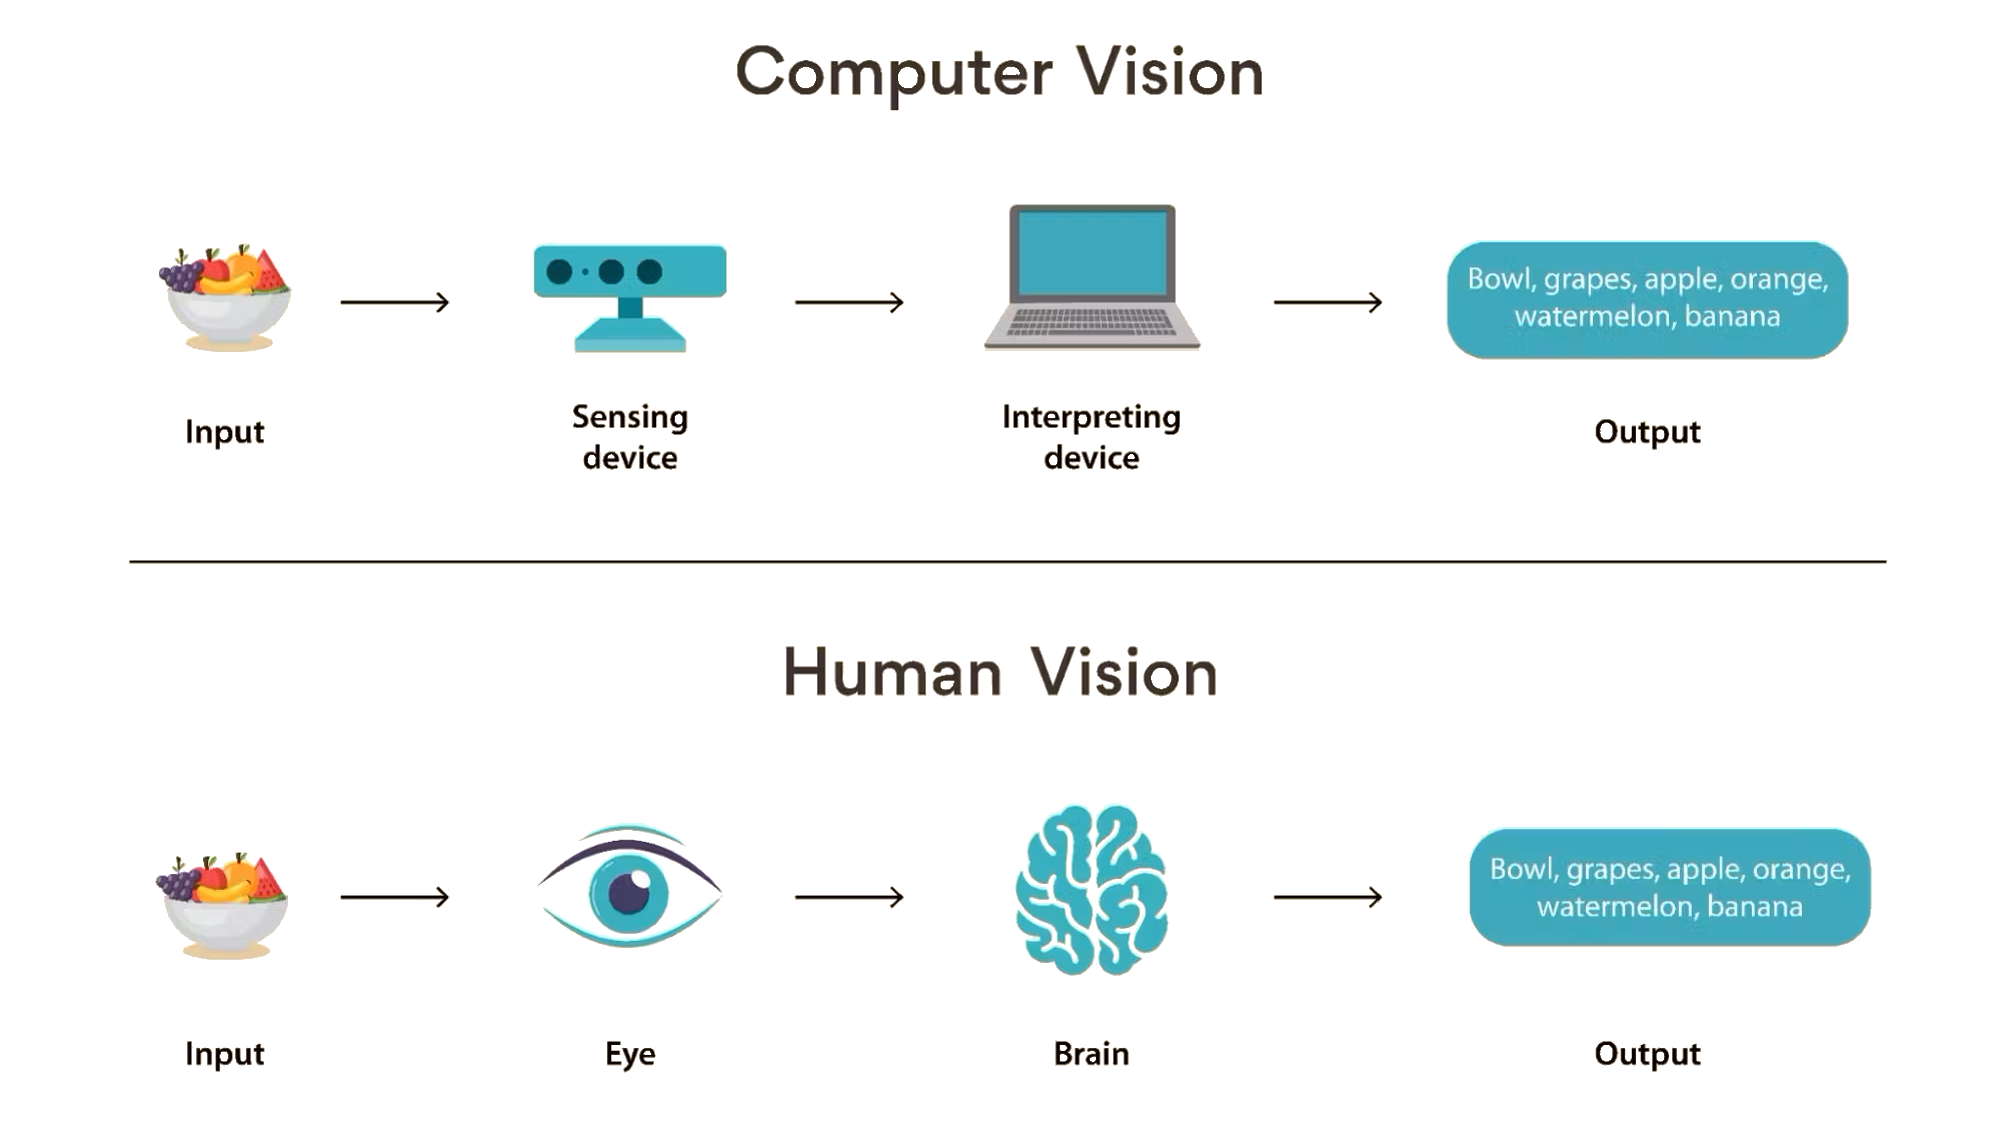
\includegraphics[width=0.75\linewidth]{figures/theory/machine-learning/computer-vision.png} \caption[Computer vision vs. human vision]{Comparison of computer vision and human vision, illustrating the similarities and differences in processing visual data \cite{turing:computer-vision}.} \label{fig:computer-vision} \end{figure}

One of the most influential technologies in modern \gls{ml} is the \gls{ann}. These networks excel at handling a wide range of data types, including images, audio, and text. Different neural network architectures are suited for specific tasks. For instance, \glspl{rnn}, especially those incorporating \gls{lstm}, are effective for sequential data such as text. \\

In contrast, \textbf{\glspl{cnn}} are particularly effective in processing image data. Their architecture leverages convolutional layers to extract spatial features. \textbf{Spatial features} refer to patterns related to the position and arrangement of pixels in an image, making \glspl{cnn} highly efficient in image classification and object detection. An example of such a network applied to handwritten digit classification is shown in Figure~\ref{fig:convolutional-neural-network}.  \\

\begin{figure}[h!] \centering 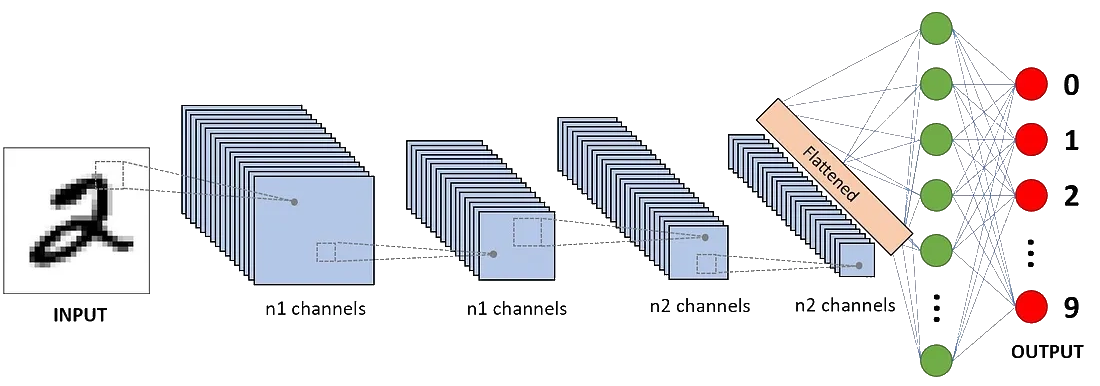
\includegraphics[width=0.75\linewidth]{figures/theory/machine-learning/convolutional-neural-network.png} \caption[CNN architecture for handwritten digit classification]{CNN architecture for classifying handwritten digits \cite{medium:cnn}.} \label{fig:convolutional-neural-network} \end{figure}

A key component of \glspl{cnn} is their ability to generate \textbf{feature maps}, which are the result of detecting spatial features at different locations in the image. These feature maps transform the input into a representation that highlights important visual patterns. As the image moves through the layers of the network, these feature maps capture crucial details such as edges, textures, and more complex shapes. Each feature map is the output of a convolutional layer, where filters are applied to extract relevant features. By emphasizing the most significant aspects of the image, these maps enable the network to learn and recognize patterns. This hierarchical approach to learning visual data has made \glspl{cnn} essential in a wide range of computer vision applications, from medical diagnostics to autonomous driving \cite{encord:cnn}. \\

Another fundamental concept in machine learning is \textbf{supervised learning}, where models are trained on labeled datasets. Each example in the dataset includes both an input and the correct output, allowing the model to learn how the input relates to the expected output. After training, the model can generalize this learned relationship to make predictions on new, unseen data \cite{geeksforgeeks:supervised-learning, google:supervised-learning}. \\

Within supervised learning, \textbf{classification} refers to predicting categorical outcomes. For example, a classification model trained on images of geometric shapes learns to associate visual features with specific shape categories. When shown a new image, the model attempts to determine the most likely category based on its prior learning. This process is illustrated in Figure~\ref{fig:supervised-learning}, which shows how labeled data is used to train a model to make accurate predictions on unseen inputs. \\

\newpage

\begin{figure}[h!] \centering 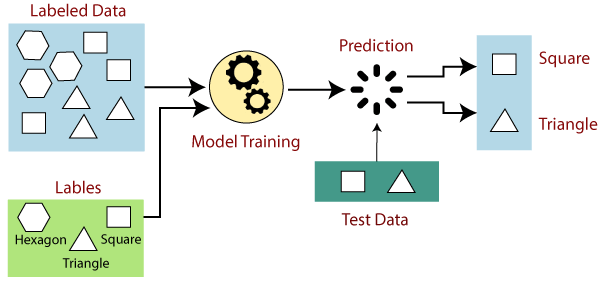
\includegraphics[width=0.75\linewidth]{figures/theory/machine-learning/supervised-learning.png} \caption[Supervised learning with labeled data]{Supervised learning process using labeled data for classification \cite{tpointtech:supervised-learning}.} \label{fig:supervised-learning} \end{figure}



By combining supervised learning with powerful models such as \glspl{cnn}, machine learning systems have achieved remarkable success in tasks that require human-like perception and decision-making \cite{chengyi:cnn}. As these models become more accurate and versatile, deploying them efficiently to real-world applications becomes increasingly important.  \\

To facilitate deployment across diverse environments and platforms, \textbf{\gls{onnx}} provides an open-source format for representing machine learning models. It enables seamless transfer and interoperability between different frameworks, including TensorFlow and PyTorch. This open format allows developers to switch between different tools depending on their specific needs during training, deployment, or optimization \cite{roboflow:onnx}.\\

Once a model is trained, \textbf{inference} is the process of using the trained model to make predictions on new, unseen data. In the context of object detection, inference involves feeding an input image into the model, which processes the image and outputs predictions, usually in the form of object classes, bounding box coordinates, and confidence scores \cite{nvidia:inference}. \\

After training and deploying a model, it is important to evaluate its performance. Two key metrics are precision and recall. \textbf{Precision} measures the proportion of correct positive predictions, indicating how many of the model’s positive predictions are actually correct. High precision means few false positives. \textbf{Recall} measures the proportion of actual positives detected by the model, showing how many relevant instances are identified. High recall means few false negatives \cite{builtin:precision-recall}.

\[
\text{Precision} = \frac{\text{True Positives}}{\text{True Positives} + \text{False Positives}}
\]

\[
\text{Recall} = \frac{\text{True Positives}}{\text{True Positives} + \text{False Negatives}}
\]

\section{Object Detection}
\label{sec:object-detection}

Object detection is a fundamental task in computer vision that involves both identifying and locating objects within an image. Unlike simple image classification, which only determines what objects are present, object detection also specifies where each object is by drawing a bounding box around it. This dual capability makes object detection essential for applications that require not just recognition, but also precise localization \cite{ibm:object-detection}. \\

\textbf{\gls{leyolo}} is a \gls{cnn}-based architecture designed for real-time object detection. It is a lightweight version of \gls{yolo} where its simplified architecture allows it to achieve faster inference times. This makes it particularly suitable for real-time applications, where quick detection is more important than achieving the highest possible accuracy. Like its predecessor, it divides an image into a grid, and each cell predicts whether an object is present, along with its bounding box coordinates \cite{openreview:leyolo}.\\

Central to object detection is the use of \textbf{bounding boxes}. Bounding boxes are rectangular regions used to indicate the location of an object within an image. It is typically represented by four values: the center coordinates \((x_c, y_c)\), which define the center of the box, and the width \((w)\) and height \((h)\), which define the dimensions of the box. In object detection tasks, models predict these coordinates to both localize and classify objects within an image \cite{peopleforai:boundingbox}. An example of how bounding boxes are used to localize objects within an image is illustrated in Figure~\ref{fig:boundingbox}.

\begin{figure}[h!]
    \centering
    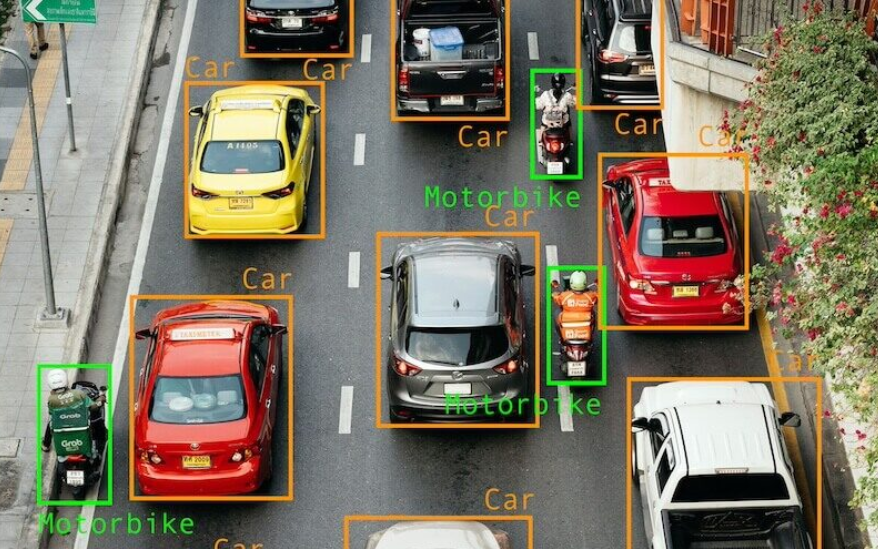
\includegraphics[width=0.75\linewidth]{figures/theory/image-recognition/bbox-example.png}
    \caption[Bounding box in object detection]{Example of a bounding boxes used in object detection to localize objects within an image \cite{peopleforai:boundingbox}.}
    \label{fig:boundingbox}
\end{figure}

To improve detection accuracy across different object sizes and shapes, models use \textbf{anchor boxes}. Anchor boxes are predefined bounding boxes of various sizes and aspect ratios, used as reference points for object detection. The sizes and aspect ratios of anchor boxes are determined by analyzing the object dimensions in the training dataset. The anchor boxes are placed over the feature map, which represents a transformed version of the input image. Rather than directly predicting bounding boxes, the model predicts offsets (shifts) relative to these anchor boxes, allowing it to adjust the box's position and size to fit the object. The model also predicts a confidence score indicating the likelihood that an object is present \cite{thinkautonomous:anchorboxes}. An illustration of how anchor boxes are positioned on the feature map is shown in Figure~\ref{fig:anchor-box}.

\begin{figure}[h!]
    \centering
    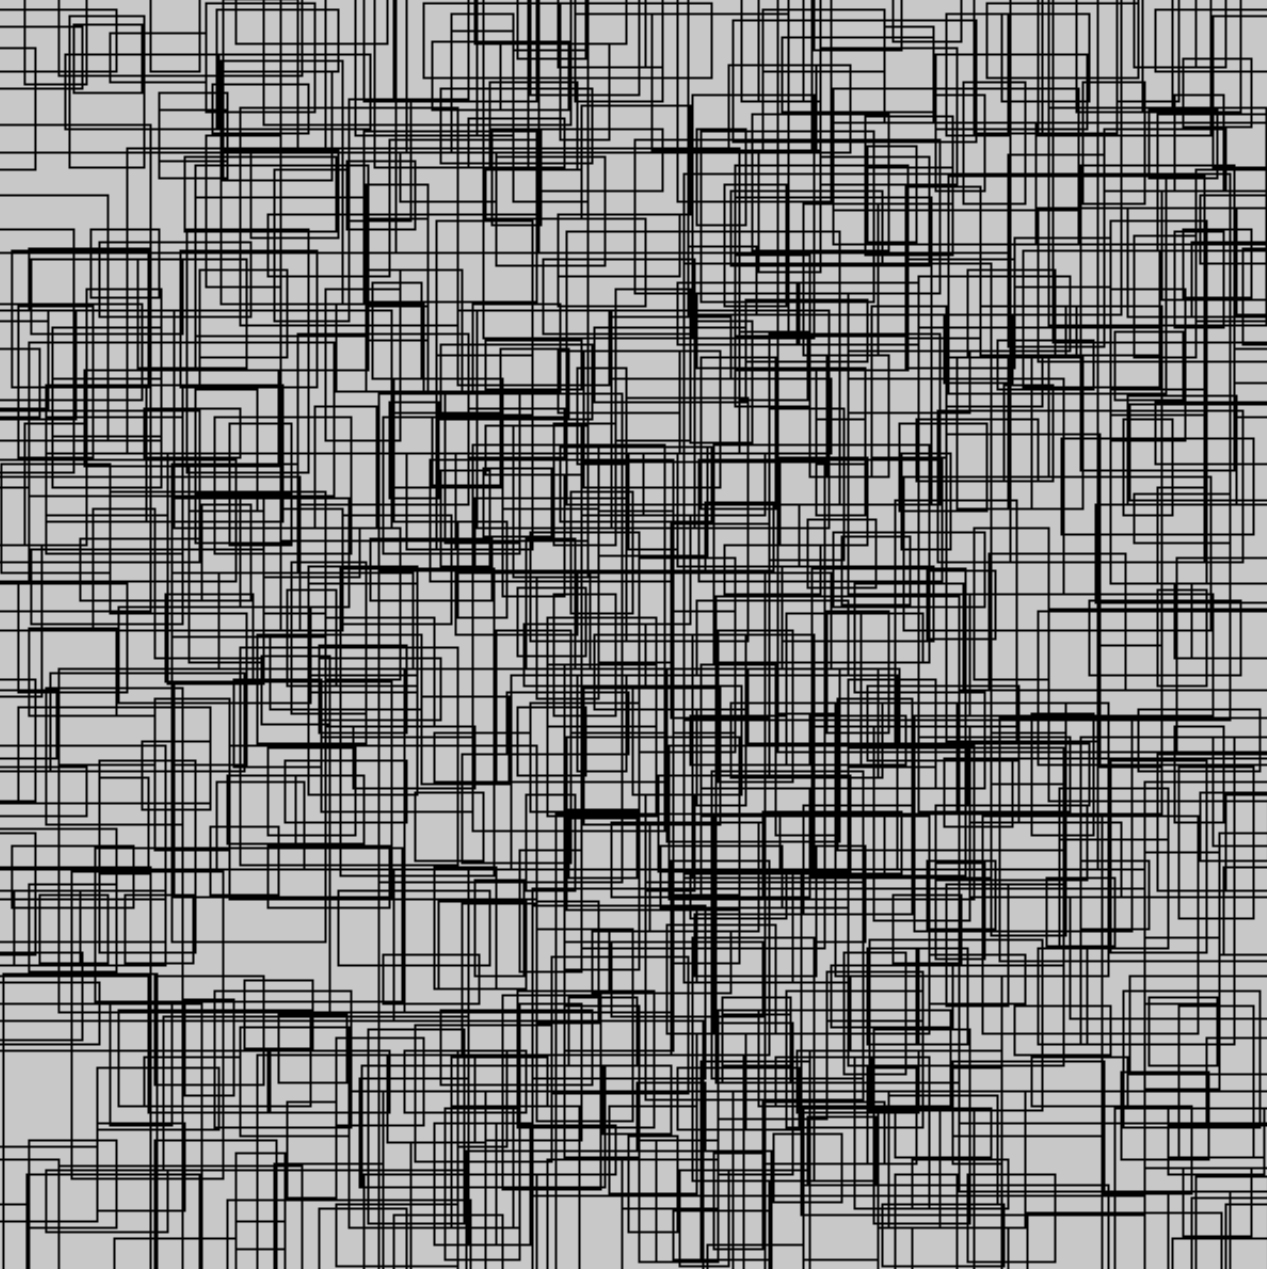
\includegraphics[width=0.7\linewidth]{figures/theory/image-recognition/anchor-boxes.png}
    \caption[Anchor boxes in object detection]{Illustration of anchor boxes on the feature map. These serve as initial reference boxes from which the model adjusts to better fit the actual objects in the image \cite{thinkautonomous:anchorboxes}.}
    \label{fig:anchor-box}
\end{figure}

To evaluate whether a predicted bounding box is accurate, a metric called \textbf{\gls{iou}} is used. \gls{iou} quantifies the overlap between the predicted bounding box and the ground truth box, the annotated box in the training dataset that precisely marks the object's true location. It is calculated as the ratio of the area of overlap to the area of union between the predicted and ground truth boxes:

\[
\text{IoU} = \frac{\text{Area of Overlap}}{\text{Area of Union}}
\]
An IoU value of 1.0 means a perfect match between the prediction and the ground truth, while 0 indicates no overlap. In practice, a prediction is considered correct if the IoU exceeds a certain threshold, commonly 0.5 \cite{ultralytics:iou}. \\

 Once multiple bounding box predictions have been made, some of them may overlap. To handle this, a post-processing technique called \textbf{\gls{nms}} is used. \gls{nms} removes redundant or overlapping bounding boxes and keeps only the most confident prediction. It selects the bounding box with the highest confidence score and suppresses all other boxes that have a high \gls{iou} overlap with it. This process repeats iteratively until no overlapping boxes remain above the chosen IoU threshold. By applying \gls{nms}, object detectors produce cleaner and more accurate results, preventing multiple detections of the same object
\cite{thepythoncode:nms}. The effect of applying \gls{nms} is illustrated in Figure~\ref{fig:nms}.

\begin{figure}[h!]
    \centering
    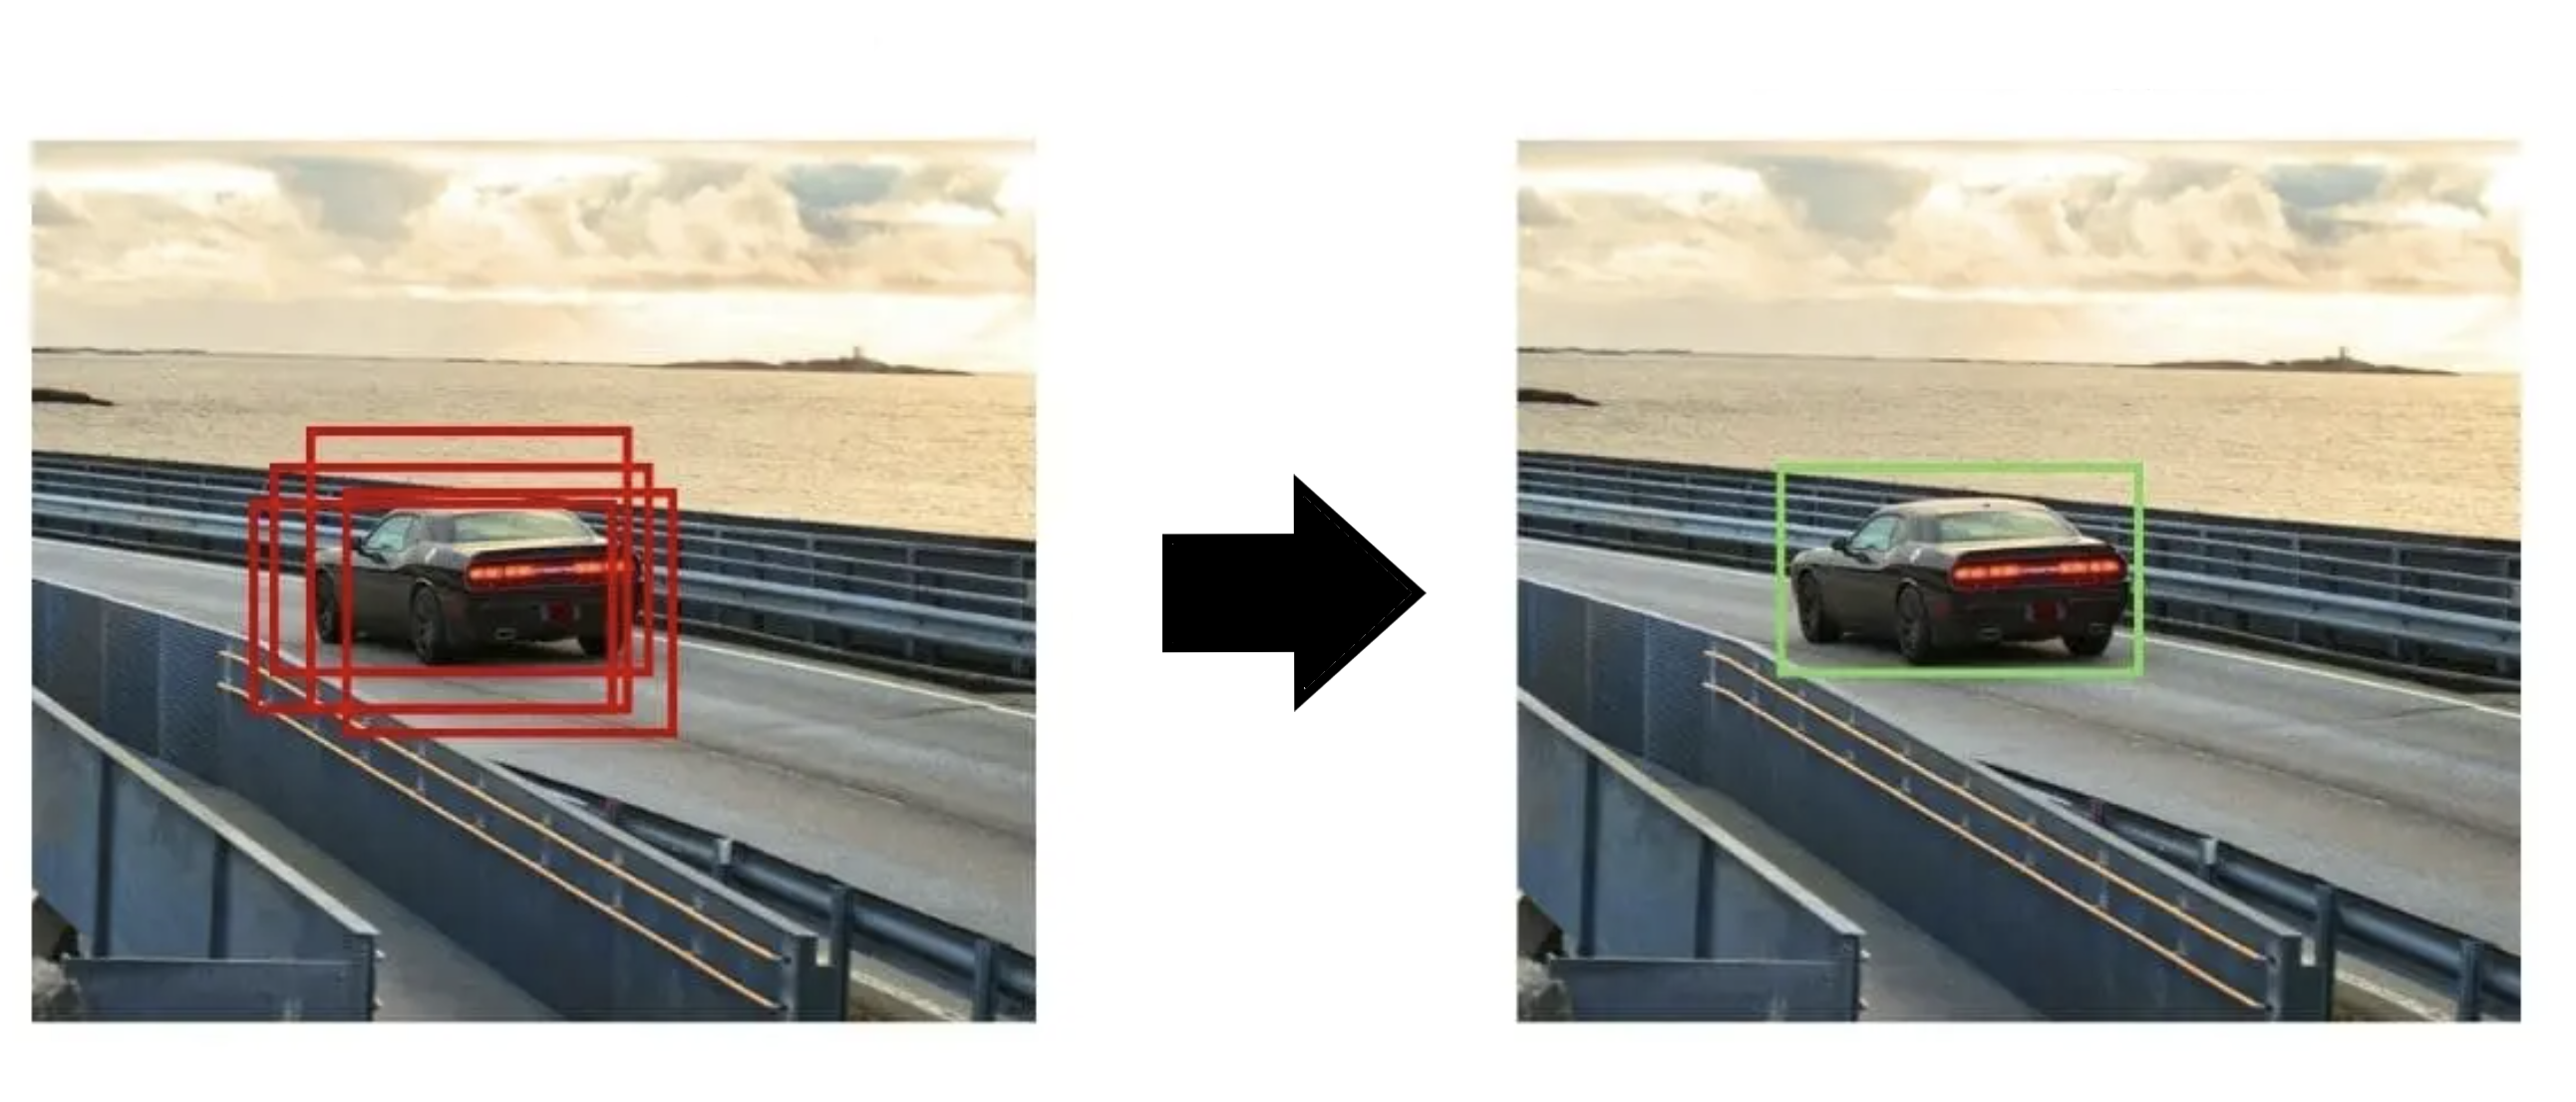
\includegraphics[width=0.75\linewidth]{figures/theory/image-recognition/nms.png}
    \caption[NMS before and after]{Illustration of NMS before and after its application \cite{thepythoncode:nms}.}
    \label{fig:nms}
\end{figure}

\section{Geometric Methods in Image Processing}
\label{sec:geometric-methods}


\subsection*{Normalization and Scaling}
\label{subsec:normalization-and-scaling}

Normalization in image processing involves adjusting pixel values to a consistent range, such as [0, 1] or [-1, 1]. This helps improve model performance by making the input data uniform. By adjusting pixel intensities from their original 0–255 range, normalization allows the model to process inputs more consistently, leading to faster and more stable convergence.
\textbf{Scaling} in image processing and machine learning involves resizing images to the format required by the model, as shown in Figure~\ref{fig:scaling} \cite{brownlee:normalization}. 

\begin{figure}[h!]
    \centering
    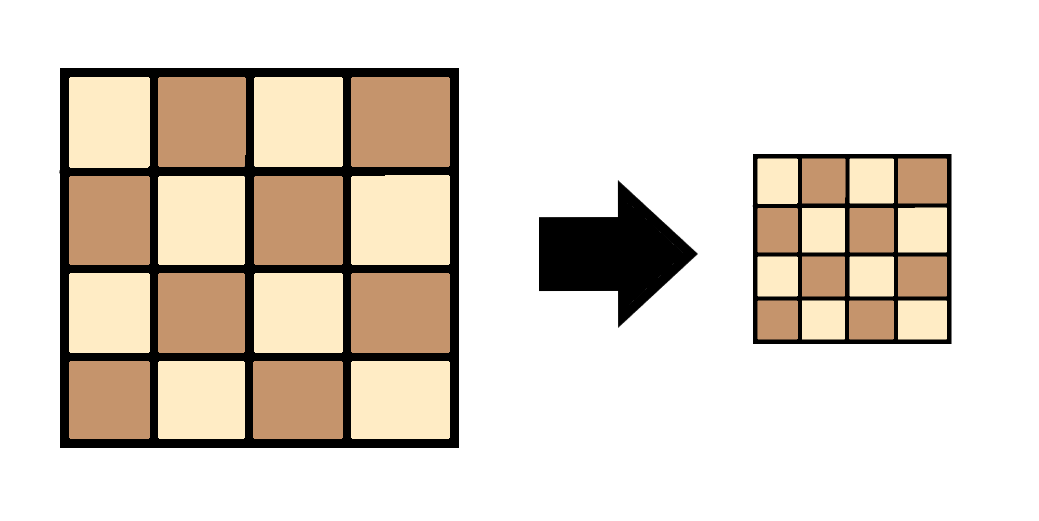
\includegraphics[width=0.75\linewidth]{figures/theory/image-recognition/scaling.png}
    \caption[Scaling before and after]{Illustration of the scaling process in image preprocessing, resizing the image to prepare it for model input.}
    \label{fig:scaling}
\end{figure}


\subsection*{Perspective Transformation}
\label{subsec:perspective-transformation}

When an image is taken from a tilted viewpoint, objects that are normally rectangular, such as chessboards, appear distorted and no longer have right angles. A perspective transformation is a specific type of image warping that corrects distortions caused by viewing a flat object from an angle. A perspective transformation uses mathematical techniques to map points from the distorted image back to their correct, undistorted positions, as illustrated in Figure~\ref{fig:perspective-transformation} \cite{nvidia:perspective-transform}.

\begin{figure}[h!]
    \centering
    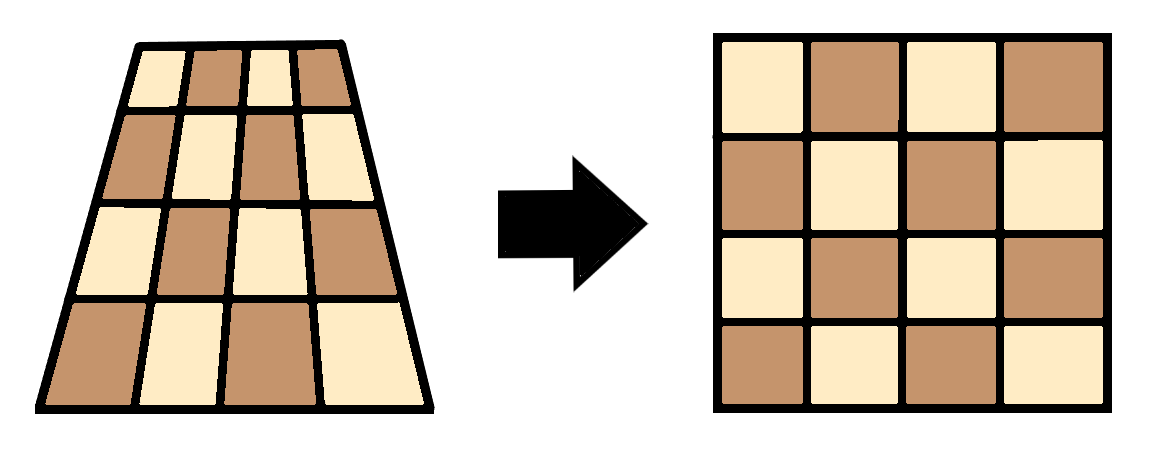
\includegraphics[width=0.75\linewidth]{figures/theory/image-recognition/perspective-transformation.png}
    \caption[Perspective transformation before and after]{Effect of perspective transformation on a distorted image. The algorithm corrects the distortion caused by an angled viewpoint, restoring the object’s original rectangular shape.}
    \label{fig:perspective-transformation}
\end{figure}

\subsection*{Euclidean Distance}
\label{subsec:euclidean-distance}

The Euclidean distance is the straight-line distance between two points in a plane. For two points with coordinates \( \mathbf{p} = (p_1, p_2) \) and \( \mathbf{q} = (q_1, q_2) \), the Euclidean distance is given by:

\[
d(\mathbf{p}, \mathbf{q}) = \sqrt{(p_1 - q_1)^2 + (p_2 - q_2)^2}
\]

This formula gives the length of the path connecting the two points. Euclidean distance is used to measure the relationship between object centers or detected positions within an image \cite{cohen:precalculus}.


\subsection*{Delaunay Triangulation}
\label{subsec:delaunay-triangulation}

Delaunay triangulation is a method of dividing a set of points into triangles such that no point is inside the circumcircle of any triangle. The circumcircle is the circle that passes through all three vertices of a triangle. It ensures that the triangles formed are as equiangular as possible,  meaning the triangle angles are close in size, minimizing the possibility of long, thin triangles. This property makes Delaunay triangulation particularly useful for applications involving geometric data, such as finding quadrilaterals from a set of points \cite{ianthehenry:delaunay}.

\section{Web}
\label{sec:web}

\subsection*{Client-Server Architecture}
\label{subsec:client-server}

Client-server architecture is a network model in which multiple clients request and receive services from a centralized server over a local network or the internet. Clients interact with the system through an application interface, while the server handles data processing. This architecture enables centralized control, scalability, and efficient resource management \cite{liquidweb:client-server}. See Figure~\ref{fig:client-server-architecture}.


\begin{figure}[h!]
    \centering
    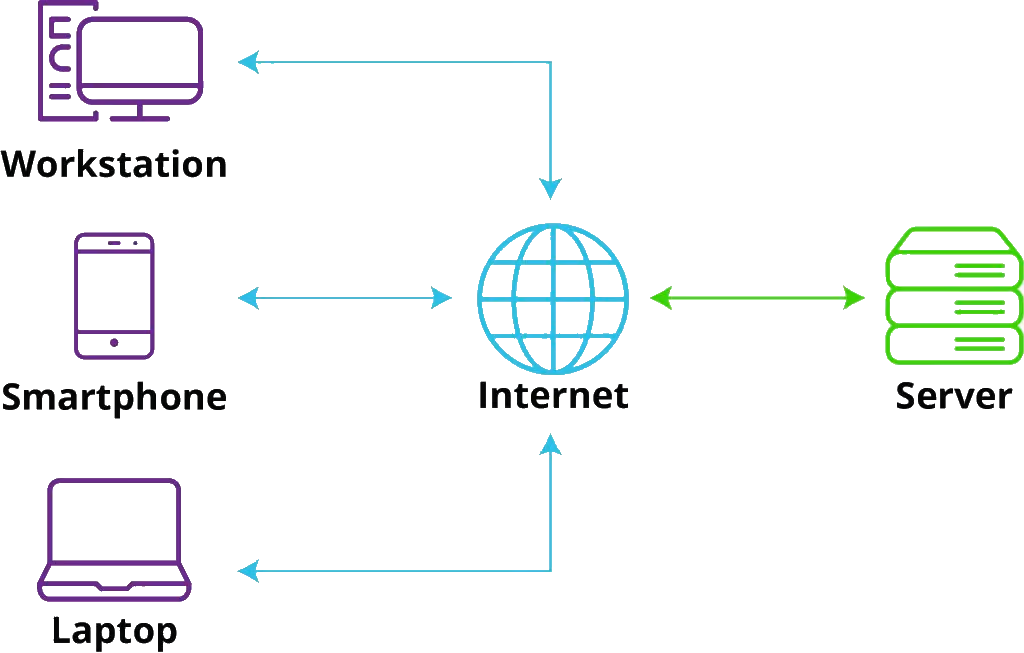
\includegraphics[width=0.75\linewidth]{figures/theory/client-server-architecture.png}
    \caption[Client-server architecture]{Client-server architecture \cite{liquidweb:client-server}.}
    \label{fig:client-server-architecture}
\end{figure}

\subsection*{WebSocket}
\label{subsec:websocket}

WebSocket is a standardized communication protocol that enables full-duplex communication over a single \gls{tcp} connection, making it well-suited for real-time web applications. Unlike traditional \gls{http} requests which follow a request-response model, WebSocket establishes a persistent connection that allows both the client and server to send and receive data at any time. This reduces the need for polling or long polling, lowering network traffic and latency. As a result, WebSocket improves the efficiency and responsiveness of data transmission, particularly in applications such as live data feeds and online games. See Figure \ref{fig:websocket-vs-http} for a comparison \cite{nodejs:websocket, apidog:websocket}.

\newpage

\begin{figure}[h!]
    \centering
    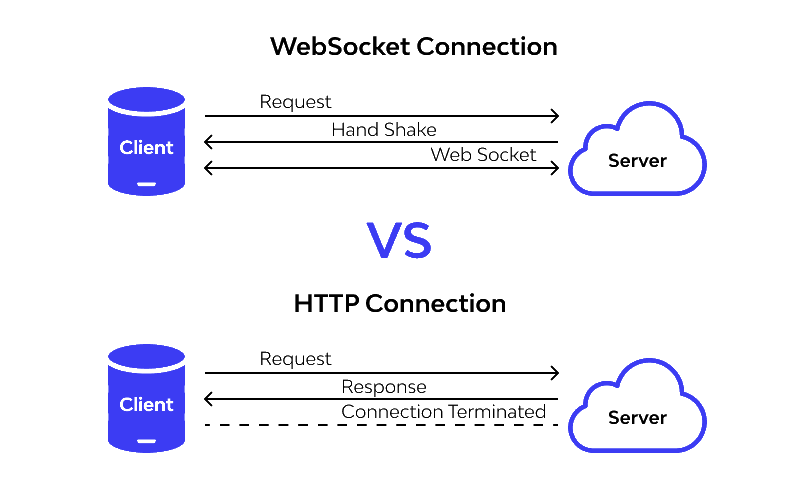
\includegraphics[width=0.70\linewidth]{figures/theory/websocket-vs-http.png}
    \caption[WebSocket connection vs. HTTP connection]{WebSocket connection vs. \gls{http} connection \cite{apidog:websocket}}
    \label{fig:websocket-vs-http}
\end{figure}

\section{Design}
\label{sec:design}

Design is a fundamental aspect of creating digital products, focusing on how users interact with and experience technology. It encompasses various disciplines, including interaction design, which aims to make digital interfaces intuitive and user-friendly. Concepts such as wireframes, accessibility, and the \gls{wcag} are often introduced to emphasize the importance of structure, usability, and universal access. \\

\textbf{Wireframes} are essential tools in the early stages of interface design. They act as simplified blueprints for websites and applications, allowing designers to plan the placement of elements such as buttons, text, and images. Wireframes enable teams to focus on layout, content structure, and user flow before any visual styling or branding is applied \cite{balsamiq:wireframe}. Separating form from function allows designers to prioritize usability and navigation before applying visual design. \\


Another essential element in design of digital solutions is \textbf{accessibility}. Universal design ensures that products are usable by as many people as possible, regardless of disabilities \cite{uutilsynet:universellutforming}. This involves considering users with visual, auditory, motor, or cognitive impairments from the beginning of the design process. By planning for accessibility early, designers not only meet legal and ethical standards, but also improve the overall user experience for everyone. Inclusive design benefits a wider audience and reduces the need for costly adaptations later in development. \\

To support accessibility in practice, the \textbf{\gls{wcag}} offer a detailed framework of recommendations. Developed by the \gls{w3c}, \gls{wcag} outlines how to make digital content more perceivable, operable, understandable, and robust \cite{levelaccess:wcag}. These guidelines are used globally to ensure web services are accessible to users with disabilities. Applying these principles from the wireframe stage onward helps integrate accessibility throughout the design process.

\section{Project Management}
\label{sec:project-management}

\textbf{Agile} is a flexible, iterative approach to managing projects, especially in software development. It emphasizes collaboration, continuous customer feedback, and the ability to quickly adapt to changing requirements throughout the project lifecycle. Agile breaks work into small, manageable increments, enabling teams to deliver value continuously and respond effectively to new information or challenges. One of the most widely used agile frameworks is \textbf{\gls{scrum}}, which organizes work into short, repeatable cycles called sprints \cite{scrumguides:scrum}. \\

\textbf{Sprints} are short time periods, usually between two and four weeks. At the start of each sprint, a meeting is held to decide the goals and how to achieve them. The objective is to complete a working piece of the product by the end of the sprint. During the sprint, a short \textbf{daily scrum meeting} is held each day to share progress and plan the next steps. At the end of the sprint, a \textbf{sprint review} is conducted to present the completed work and gather feedback. Additionally, a \textbf{sprint retrospective} is held to reflect on what went well, identify areas for improvement, and define actions to enhance the workflow for the next sprint. \\

\gls{scrum} uses three main artifacts to organize and manage the work process. The \textit{product backlog} is a list of all features, enhancements, and fixes planned for the product. The \textit{sprint backlog} contains the specific tasks selected for implementation during the current sprint. Finally, the \textit{increment} is the completed, usable product delivered at the end of the sprint. Together, these artifacts promote transparency, align team efforts, and ensure consistent progress throughout the development cycle \cite{scrumguides:scrum}. \\

Scrum has three primary roles. The \textbf{product owner} is responsible for deciding what the team should work on and in what order. The \textbf{development team} builds the product and takes ownership of organizing and completing the work. The \textbf{scrum master} facilitates the process by supporting the team, removing obstacles, and ensuring that scrum practices are followed effectively.\\

\section{Software Engineering Principles}
\label{sec:software-engineering-principles}

\subsection{Code Review}
\label{subsec:code-review}

Code review is a process in which one or more developers examine another developer’s code before it is merged into a shared branch, such as the main branch. The purpose is to identify issues such as bugs, logic errors, or edge cases that may not have been caught during initial development \cite{gitlab:code-review}. \\

Modern version control systems often use pull requests to facilitate code reviews. A pull request is a formal proposal to merge changes from one branch into another and provides a platform for reviewing, discussing, and approving code. It also highlights differences between branches, helping reviewers understand and evaluate the proposed changes \cite{github:pr}.

\subsection{Cohesion and Coupling}
\label{subsec:cohesion-and-coupling}

\begin{quote}
\textit{"\textbf{Cohesion} refers to the degree to which elements within a module work together to fulfill a single, well-defined purpose. \textbf{High cohesion} means that elements are closely related and focused on a single purpose, while \textbf{low cohesion} means that elements are loosely related and serve multiple purposes."} \cite{geeksforgeeks:c&c} \\
\end{quote}

\begin{quote}
\textit{"\textbf{Coupling} refers to the degree of interdependence between software modules. \textbf{Tight coupling} means that modules are closely connected and changes in one module may affect other modules. \textbf{Loose coupling} means that modules are independent, and changes in one module have little impact on other modules."} \cite{geeksforgeeks:c&c} \\
\end{quote}

\begin{figure}[h!]
    \centering
    \subfloat{{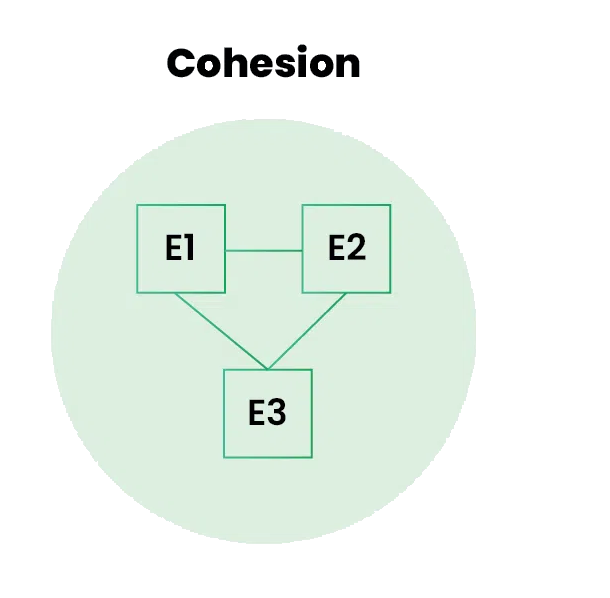
\includegraphics[width=0.5\linewidth]{figures/theory/cohesion.png}}}
    \subfloat{{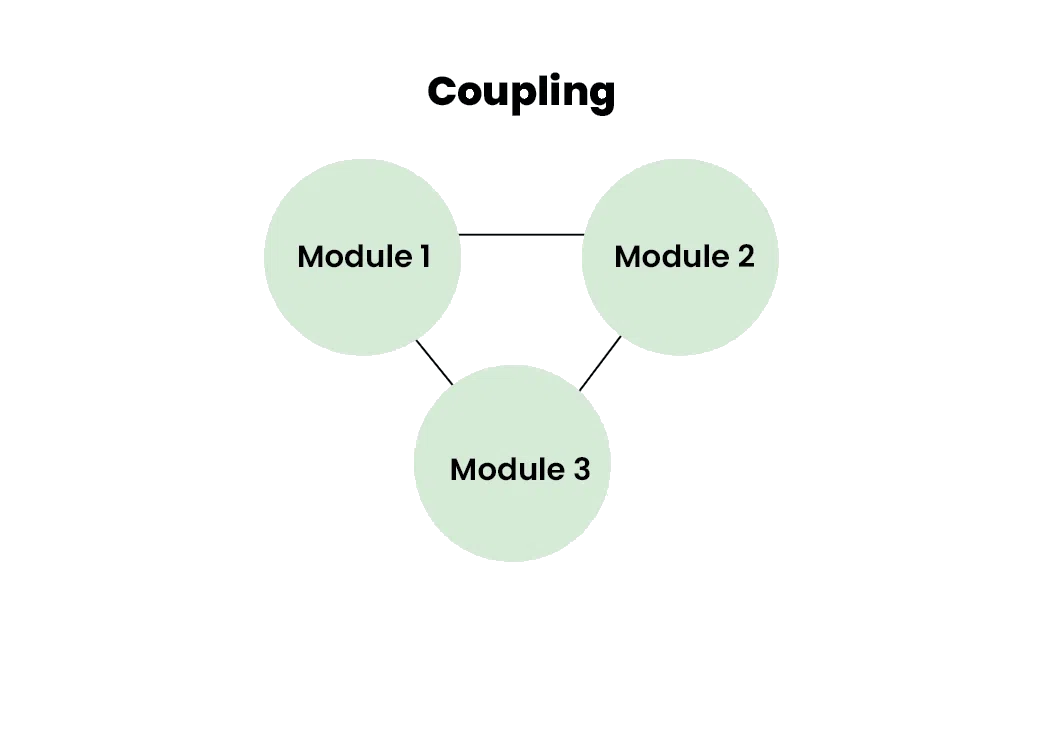
\includegraphics[width=0.5\linewidth]{figures/theory/coupling.png}}}

    \caption[Cohesion and coupling]{Cohesion and coupling \cite{geeksforgeeks:c&c}}
    \label{fig:cohesion-coupling}
\end{figure}

Cohesion and coupling impact the quality and maintainability of a system.
High cohesion and loose coupling are desirable, as they lead to systems that are easier to test, modify, and extend. This relationship is illustrated in Figure \ref{fig:cohesion-coupling} 
\cite{geeksforgeeks:c&c}.

\subsection{Documentation}
\label{subsec:documentation}

Documentation is an essential part of software development, providing written references for developers, testers, and users. It includes materials such as \gls{api} references, build instructions, user guides, and design specifications. Documentation supports understanding, maintenance, and helps preserve knowledge over time. It should be created and maintained alongside the code to stay accurate and useful throughout the project lifecycle \cite{geeksforgeeks:doc}.

\subsection{Testing}
\label{subsec:testing}

\subsubsection*{Virtual Machine}
\label{subsubsec:virtual-machine}

A \gls{vm} is a software program that acts like a real computer. It runs on a physical machine (the host) and has its own virtual \gls{cpu}, memory, and storage. The \gls{vm} is separated from the host system, so anything running inside the \gls{vm} cannot directly affect the host. This makes it useful for testing, running different operating systems, or isolating software environments \cite{microsoft:virtual-machine}.

\subsubsection*{Unit Testing}
\label{subsubsec:unit-testing}

Unit testing involves testing individual components of a software application in isolation, such as functions, methods, or classes. The purpose is to ensure that each unit behaves as expected and is reliable under different conditions \cite{geeksforgeeks:unit-test}.

\subsubsection*{Usability Testing}
\label{subsec:usability-testing}

Usability testing evaluates a system from the end user’s perspective, focusing on how easily users can interact with the system to accomplish their goals. It involves observing users to identify areas of confusion, inefficiency, or difficulty in the user experience \cite{geeksforgeeks:user-test}.

Both qualitative data (e.g., user feedback) and quantitative data (e.g., task completion rates) are collected to assess functionality and user satisfaction. These findings are used to generate a report with recommendations for improving usability \cite{geeksforgeeks:user-test}.

\subsection{Type Safety}
\label{subsec:type-safety}

Type safety ensures that operations in a program are performed on the correct data types, helping catch errors early in development. In dynamically typed languages like JavaScript, lack of type enforcement can lead to hidden bugs. Enforcing type safety reduces runtime errors and improves code reliability \cite{dev:type-safety}.

\subsubsection*{Key Pillars of Type Safety}
\label{subsubsec:type-safety-pillars}

\begin{itemize}
\item \textbf{Reliability:} Enforcing correct data types prevents type-related runtime errors, improving application stability \cite{dev:type-safety}.

\item \textbf{Collaboration:} Clear type definitions make code easier to read and understand, aiding teamwork and maintainability \cite{dev:type-safety}.

\item \textbf{Efficient Debugging:} Detecting type errors early reduces debugging time and lowers the risk of runtime issues \cite{dev:type-safety}.
\end{itemize}
